\chapter{Forretningsanalyse}
\label{chapter:forretningsanalyse}

Dette kaptitel indeholder en forretningsanalyse af Blomsterbinderiet, der er en blomsterbutik, der er beliggende i Meny i en større dansk provinsby.
I \ref{chapter:conclusion} forefindes afsnittet \ref{sec:conclusion_summary}, der opsummerer hele afsnittet og dens anvendelse i projektet.

\section{Analyse af forretningsmodel}
Butikken er bemandet af faguddanet personel, der har stor erfaring med at sammensætte buketter og dekorationer. 
Fysisk er de placeret i Meny, hvilket giver dem en fordel i forhold til kunder, der handler i supermarkedet og ser butikken. Ydermere ligger de ud til gågaden og der er en parkeringsplads på bagsiden af butikken, hvilket tilføjer til kundegennemstrømning. 
Samtidig er er tilstede på sociale medier, hvilket giver dem en mulighed for at nå ud til flere kunder.
Personalet har et stort fokus på at inspirere kunderne til at købe blomster, fx. ved at have dekorationer, der passer til mærkedage og sæsoner. 
Butikken har en relativt stor kundegruppe, der er loyale overfor butikken og de har et samarbejde med bedemænd, hvilket giver dem en fast indtægt. 
Butikken er de ejet af Meny, hvilket giver dem en økonomisk bund, der er større end andre blomsterbutikker.
Der er en kulturel forventning om at give blomster i sociale sammenhænge, hvilket giver mere robusthed ift. økonomiske konjukturer.

Der er dog nogle svagheder ved butikken. 
Der er ingen reelle IT-kompetencer in-house, så vedligeholdelse af deres hjemmeside, vil være en ekstern opgave, der gør dem afhængig af en form for IT-leverandør.
Det medfører også, at et evt. IT-system, skal være både brugervenligt og stabilt, så butikken selv kan oprette produkter m.m. 
Der skelnes her mellem indhold på websitet og selve systemet bag, så vedlighold i den her sammenhæng vil bl.a. indebære at systemet porteres til en nyere .NET version.
Butikken ligger inde i Meny, hvilket kan få kunder til at tænke at de sælger supermarkedsblomster, hvilket kan give en opfattelse af lavere kvalitet.
Butikken har svært ved at opbygge et varelager, da blomster har en kort holdbarhed.
Butikkens kolokering med Meny kan gøre, at folk ikke opfatter at butikken er selvstændig.
Butikken har ingen online tilstedeværelse, hvilket gør det svært for dem at nå ud til kunder, der ikke handler i Meny.

Der er nogle muligheder for butikken. Der er en stigende kvalitetsbevidsthed i befolkningen, hvilket kan give butikken mulighed for at sælge flere blomster.
Der er en stigning i antallet af importerede mærkedage, fx. valentinsdag, hvilket kan give butikken mulighed for at sælge flere blomster.
Folk arbejder mere hjemme, hvilket kan give butikken mulighed for at sælge flere blomster til hjemmet.
Butikken kan udvide samarbejdet med bedemænd, hvilket kan give dem en fast indtægt.
Butikken kan udvide deres samarbejde med andre virksomheder, fx. kontorer, eventsteder, restauranter/caféer, hvilket kan give dem en fast indtægt.

Der er dog også nogle trusler for butikken. Butikken er afhængig af globale supply lines (bl.a. tulipaner fra Holland), hvilket kan gøre det svært for dem at opretholde deres varelager.
En forværring af den nuværende økonomiske situation, fx. en økonomisk depression, kan få folk til at købe færre ikke-essentielle produkter, hvilket kan påvirke butikkens indtjening.
Der er konkurrence fra andre blomsterbutikker, der også er på sociale medier og har deres egen hjemmeside.
Det er et mættet marked, hvilket kan gøre det svært for butikken at tiltrække nye kunder.

\section{SWOT}
For at opsummere og kondensere de mest relevante dele af forretningsanalysen, er der udfærdiget en SWOT analyse for Blomsterbinderiet.
\begin{table}[H]
    \centering
    \begin{tabular}{|
        >{\bfseries\columncolor[HTML]{68CBD0}}m{0.7cm}|
        >{\columncolor[HTML]{68CBD0}}m{6.8cm}|
        >{\columncolor[HTML]{68CBD0}}m{6.8cm}|}
    \hline
     & \textbf{Positive} & \textbf{Negative} \\ \hline
    \textbf{Int.} & 
    Styrker:
    \begin{itemize}
        \item Faguddannet personale
        \item Beliggenhed i Meny
        \item SoMe tilstedeværelse
        \item Stabilt samarbejde med bedemænd
        \item Økonomisk støtte fra Meny
    \end{itemize} & 
    Svagheder:
    \begin{itemize}
        \item Ingen IT-kompetencer in-house
        \item Neglicierbart varelager
        \item Afhængig af Meny
        \item Ingen nuværende webshop
    \end{itemize} \\ \hline
    \textbf{Ext.} & 
    Muligheder:
    \begin{itemize}
        \item Stigende kvalitetsbevidsthed
        \item Øget efterspørgsel fra hjemmearbejde
        \item Mulighed for udvidelse af samarbejder
        \item Udvikling af webshop
    \end{itemize} & 
    Trusler:
    \begin{itemize}
        \item Afhængighed af globale supply lines
        \item Potentiel økonomisk nedgang
        \item Konkurrence fra andre blomsterbutikker
        \item Mættet marked
    \end{itemize} \\ \hline
    \end{tabular}
    \caption{SWOT Analyse for Blomsterbinderiet}
    \label{tab:swot}
\end{table}

\section{Business Model Canvas}
Der er ligeledes udfærdiget et Business Model Canvas for Blomsterbinderiet, der kan bruges til at give et andeerledes overblik over de vigtigste aspekter af forretningsmodellen.
\begin{figure}[H]
    \centering
    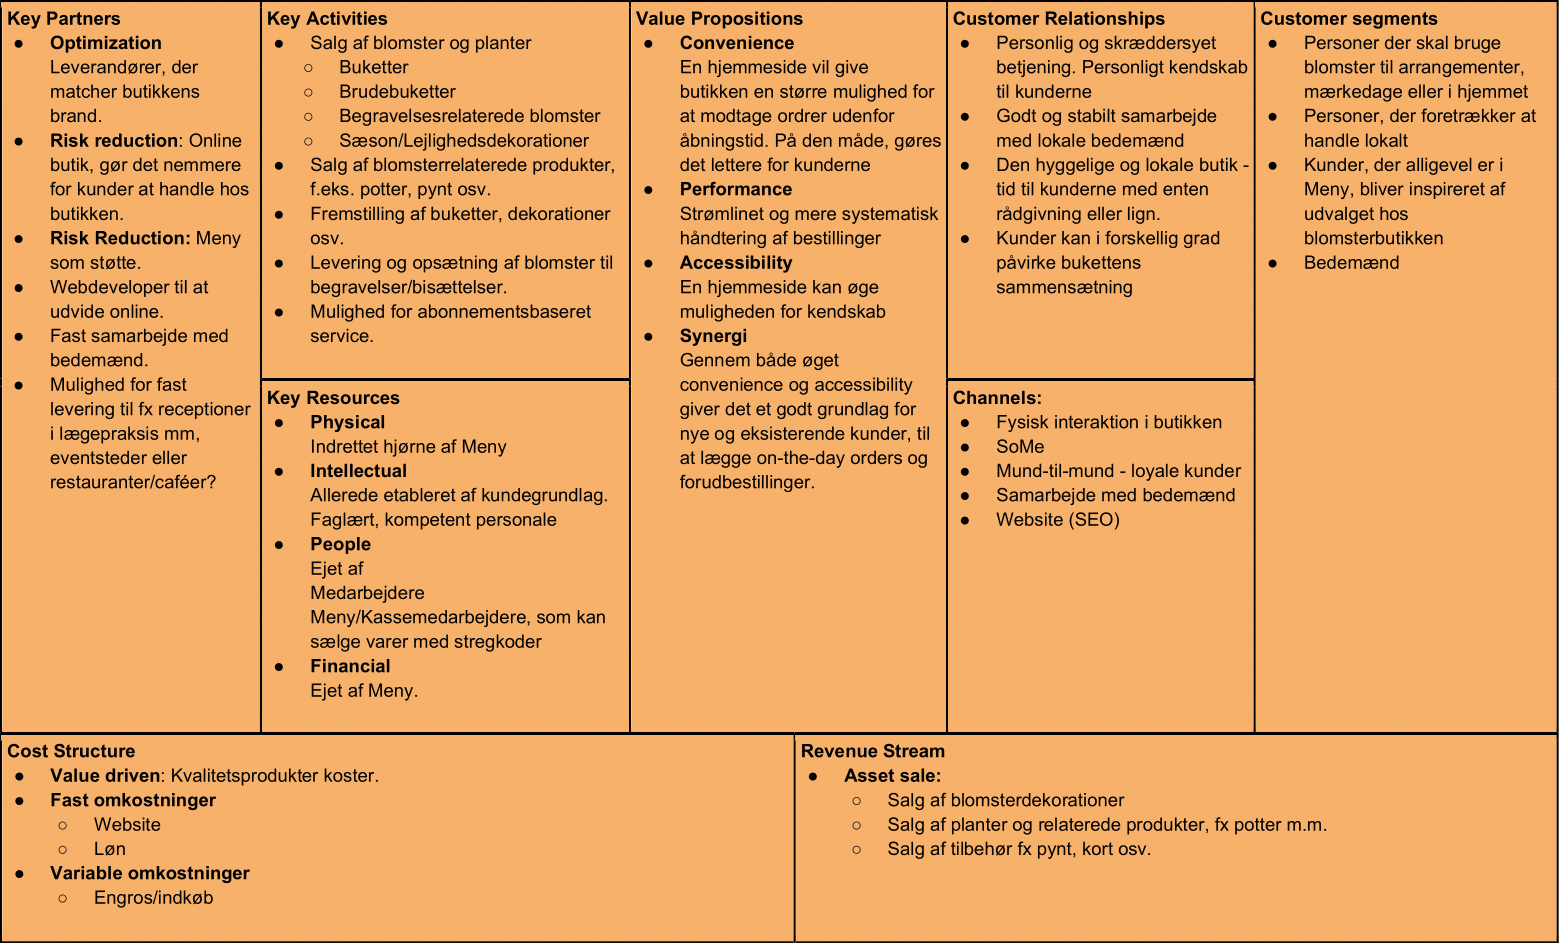
\includegraphics[width=1\textwidth]{figures/business/bmc1.png}
    \caption{Business Model Canvas for Blomsterbinderiet}
    \label{fig:bmc1}
\end{figure}

\section{Inception Deck}

\subsection{Why are we here?}
Vi vil skabe en online platform for Blomsterbinderiet, der vil transformere måden, 
hvorpå butikken kan interagere med kunder og bedemænd, ved at tilbyde en brugervenlig, 
informativ og æstetisk tiltalende webshop, styrket af personlig og effektiv service.

\subsection{Elevator Pitch}
Til blomsterbutikken, der ønsker at levere den bedste oplevelse indenfor blomsterdekorationer, 
har vi udviklet en online platform, der gør det nemt for både private og erhverv at få blomster, buketter etc, der er skræddersyet til deres behov.
Dette vil understøtte butikkens eksisterende forretning, muliggøre en udvidelse af kundegruppen samt give yderligere mulighed for at yde god service.
Selvom vores platform er online, vil den i modsætning til konkurrenterne være forankret i det lokale og den personlige service.

\subsection{Product Box}
Sammen med mockups og wireframes, er der udarbejdet en Product Box, der kan bruges til at give et overblik over produktet \ref{fig:product-box}.
\begin{figure}[H]
    \centering
    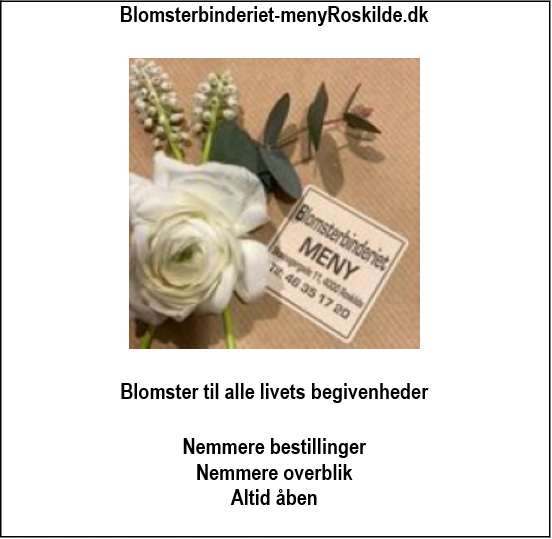
\includegraphics[width=0.4\textwidth]{figures/business/product-box.png}
    \caption{Product Box for Blomsterbinderiet}
    \label{fig:product-box}
\end{figure}

\subsection{NOT List}
For at skabe klarhed over, hvad der er i scope og hvad der er out of scope, er der udarbejdet en NOT List \ref{tab:not-list}.
\begin{table}[H]
    \centering
    \begin{tabular}{|
    >{\columncolor[HTML]{DAE8FC}}l 
    >{\columncolor[HTML]{DAE8FC}}l |}
    \hline
    \multicolumn{1}{|c|}{\cellcolor[HTML]{DAE8FC}\textbf{In Scope}}                                                                                                                                                                                                                                                                                           & \multicolumn{1}{c|}{\cellcolor[HTML]{DAE8FC}\textbf{Out of Scope}}                                                                       \\ \hline
    \multicolumn{1}{|l|}{\cellcolor[HTML]{DAE8FC}\begin{tabular}[c]{@{}l@{}}Website med modeller for produkter m.m.\\ Filtrering og sortering af udvalgte modeller\\ CRUD på udvalgte modeller\\ Database til at gemme modellerne\\ Kurv funktion\\ Ordre funktion\\ Authentication funktionalitet\\ Analyse af data fra website\end{tabular}} & \begin{tabular}[c]{@{}l@{}}Advanced security features\\ Webhosting\\ Email notifications\\ Website statestik, fx Google API\end{tabular} \\ \hline
    \multicolumn{2}{|c|}{\cellcolor[HTML]{DAE8FC}\textbf{Unresolved}}                                                                                                                                                                                                                                                                                                                                                                                                                                    \\ \hline
    \multicolumn{2}{|l|}{\cellcolor[HTML]{DAE8FC}\begin{tabular}[c]{@{}l@{}}Søgning i produkter gennem Keywords\\ Content Management System\end{tabular}}                                                                                                                                                                                                                                                                                                                                                \\ \hline
    \end{tabular}
    \caption{NOT List}
    \label{tab:not-list}
\end{table}

\subsection{Meet your neighbors}
Butiksejeren/bestyreren, der er projektets kunde (stakeholder), giver input til forretningsgang, designønsker m.m.
Personalet er de ansatte i butikken, der skal bruge platformen til at modtage og ekspedere ordre, samt kunne levere service.
Kunderne er primært private, der ønsker at købe blomster til forskellige begivenheder, fx. fødselsdage, bryllupper, begravelse etc.
Bedemændene er erhvervskunder, der ønsker at købe blomster og services ifm. begravelser.
Meny er butikkens ejer og samarbejdspartner.
Leverandørerne, der leverer blomster til butikken, er hovedsageligt et mellemled til det globale marked.
Technical/Internal Product Owner rollen vil i det her projekt blive varetaget af mig, da jeg er den eneste udvikler. Det vil afsøges om en lektor kan indgå som Product Owner til nogle sessioner.

\subsection{Show the solution}
Den foreslåede teknologiske stack og overordnede arkitektur, der skal implementeres \ref{fig:show-the-solution}. 
\begin{figure}[H]
    \centering
    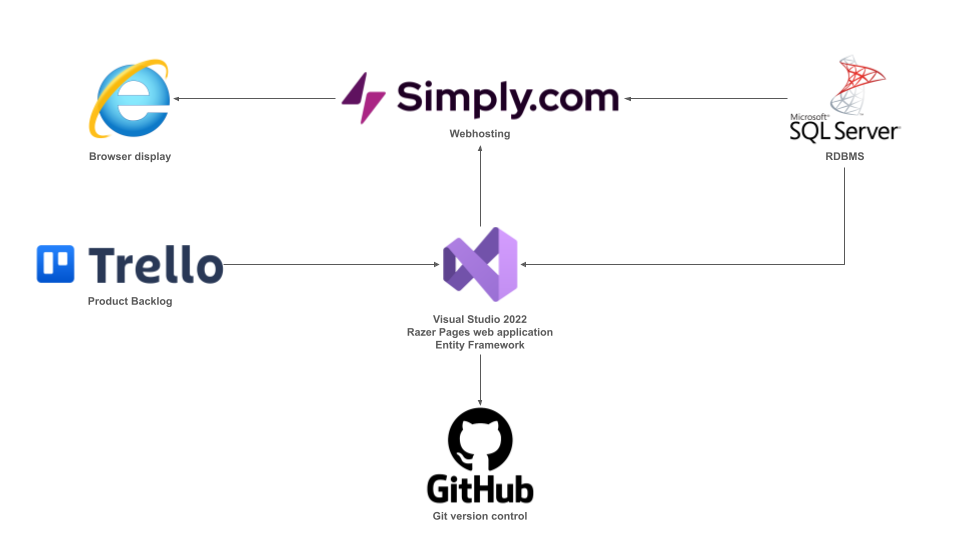
\includegraphics[width=0.75\textwidth]{figures/business/show-the-solution.png}
    \caption{The solution - billeder fra \cite{1000logos}}
    \label{fig:show-the-solution}
\end{figure}

\subsection{What keeps us up at night}
Der er identificeret nogle risikofaktorer, angivet i sandsynlighed (S) og alvorlighed (A) på en skala fra 1 til 5, hvor 1 er det laveste \ref{tab:risiko-analyse}.
\begin{table}[H]
    \centering
    \begin{tabular}{|
    >{\columncolor[HTML]{FFCCC9}}m{4.2cm} |
    >{\columncolor[HTML]{FFCCC9}}m{0.6cm} |
    >{\columncolor[HTML]{FFCCC9}}m{0.6cm} |
    >{\columncolor[HTML]{FFCCC9}}m{8.5cm} |}
    \hline
    \textbf{Risiko}             & \textbf{S} & \textbf{A} & \textbf{Mitigations Strategi}                                                                                      \\ \hline
    Begrænset tid til projektet & 5          & 5          & Der stiles mod et MVP tidligt i processen. Tasks prioriteres gennem SCRUM og der scope skaleres \\ \hline
    Tekniske udfordringer       & 4          & 3          & Projektets scope afgrænses, try-and-throw mindset og der søges ekspertviden     \\ \hline
    Begrænset personel          & 5          & 3          & Der er kun én udvikler på projektet. En disciplineret indsats er nødvendig                     \\ \hline
    For lav velocity            & 3          & 3          & Såfremt burndown chart angiver en for lav velocity, vil efterfølgende sprints rekonstrueres                  \\ \hline
    \end{tabular}
    \caption{Risiko analyse}
    \label{tab:risiko-analyse}
\end{table}

\subsection{Size it up}
Deadline er 30. maj 2024, som giver denne overordnede tidsplan \ref{list:size-it-up}.
\begin{itemize}[noitemsep]
    \item Sprint 0: 1 uge, sammenfatte og redigere eksisterende materiale
    \item Sprint 1-5: 5 uger i alt til udvikling. Der er afsat 37 timer pr. sprint
    \item Afsluttende uge: 1 uge til at sammenfatte rapporten etc
    \label{list:size-it-up}
\end{itemize}

\subsection{What is going to give}
I stedet for de klassiske sliders, er der udarbejdet en rangeret liste over features og fokusområder \ref{list:what-is-going-to-give}. 
Som på en stack er de øverste også de første, der vil blive poppet af, hvis der opstår problemer.
\begin{enumerate}[noitemsep]
    \item Website statestik, fx Google API
    \item Advanced security features
    \item Website performance optimization
    \item Email notifications
    \item Content Management System
    \item Webhosting
    \item Test (Unit test etc.)
    \item Design and layout
    \item Restrictions and requirements
    \item Søgning i produkter gennem Keywords
    \item Analyse af data fra website
    \item Kurv funktion
    \item Ordre funktion
    \item Filtrering og sortering af udvalgte modeller
    \item CRUD på udvalgte modeller
    \item Authentication funktionalitet
    \item Database til at gemme modellerne
    \item Website med modeller for produkter, ordre, kunder m.m.
    \label{list:what-is-going-to-give}
\end{enumerate}

\subsection{What it's going to take}
Grundet projektets natur er budgettet irrelevant og der vil ikke blive tilført flere udviklere.
Den eneste håndta der kan skrues på er antal timer brugt på projektet, frem mod deadline.